\documentclass{article}
\setlength{\headheight}{13.6pt}
\usepackage[margin=1in]{geometry}
\usepackage{amsmath, amssymb, amsfonts}
\usepackage{graphicx}
\usepackage{tikz}
\usepackage{hyperref}
\usepackage{booktabs}
\usepackage{array}
\usepackage{float}
\usepackage{caption}
\usepackage{subcaption}
\usepackage{tcolorbox}
\usepackage{xcolor}
\usepackage{titlesec}
\usepackage{fancyhdr}
\usepackage{colortbl}
\usetikzlibrary{shapes,arrows,positioning,fit,calc}

% Custom colors - all black/grayscale with contrast
\definecolor{myorange}{rgb}{0.3, 0.3, 0.3}
\definecolor{myblue}{rgb}{0.2, 0.2, 0.2}
\definecolor{mygreen}{rgb}{0.25, 0.25, 0.25}
\definecolor{myred}{rgb}{0.35, 0.35, 0.35}
\definecolor{buetgreen}{rgb}{0.0, 0.0, 0.0}
\definecolor{darkcharcoal}{rgb}{0.2, 0.2, 0.2}
\definecolor{lightgray}{rgb}{0.92, 0.92, 0.92}
\definecolor{mediumgray}{rgb}{0.85, 0.85, 0.85}
\definecolor{highlight}{RGB}{255, 255, 153}

% Title formatting
\titleformat{\section}{\large\bfseries\color{black}}{\thesection}{1em}{}
\titleformat{\subsection}{\normalsize\bfseries\color{black}}{\thesubsection}{1em}{}

% Header/Footer
\pagestyle{fancy}
\fancyhf{}
\fancyhead[L]{\small Hierarchical Clustering}
\fancyhead[R]{\small CSE200 - Technical Writing and Presentation}
\fancyfoot[C]{\thepage}

% Change tcolorbox to plain boxes with visible headings
\tcbset{
    sharp corners,
    boxrule=0.5pt,
    colback=white,
    colframe=black,
    colbacktitle=black!15,
    coltitle=black,
    fonttitle=\bfseries
}


\begin{document}

% ============================================================
% TITLE PAGE
% ============================================================
\begin{titlepage}
    \centering
    \vspace*{1cm}
    
    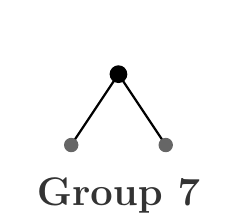
\begin{tikzpicture}[scale=0.6]
        \draw[black, thick] (0,1.5) -- (-1,0);
        \draw[black, thick] (0,1.5) -- (1,0);
        \filldraw[black] (0,1.5) circle (5pt);
        \filldraw[black!60] (-1,0) circle (4pt);
        \filldraw[black!60] (1,0) circle (4pt);
        \node[below, black!80, font=\Large\bfseries] at (0,-0.5) {Group 7};
    \end{tikzpicture}
    
    \vspace{0.5cm}
    
    {\large \textbf{BANGLADESH UNIVERSITY OF ENGINEERING AND TECHNOLOGY}} \\
    {\large \textbf{Department of Computer Science and Engineering}}
    
    \vspace{1.5cm}
    
    {\Huge \textbf{\textcolor{black}{Hierarchical Clustering}}} \\
    \vspace{0.3cm}
    {\Large \textit{Building a Family Tree for Your Data}}
    
    \vspace{1.5cm}
    
    \begin{tabular}{ll}
        \textbf{Section} & : B2 \\
        \textbf{Group}   & : 07 \\
        \textbf{Date}    & : \today \\
    \end{tabular}
    
    \vspace{1.5cm}
    
    \begin{tabular}{ll}
        \textbf{Apurbo Das Pranto}   & ID: 2205091 \\
        \textbf{Mahrez Hussain Khan} & ID: 2205109 \\
        \textbf{Md. Tanveer Hossain} & ID: 2205112 \\
    \end{tabular}
    
\end{titlepage}

% ============================================================
% TABLE OF CONTENTS
% ============================================================
\tableofcontents
\newpage

% ============================================================
% LIST OF FIGURES
% ============================================================
\listoffigures
\newpage

% ============================================================
% ABSTRACT
% ============================================================
\section*{Abstract}
\addcontentsline{toc}{section}{Abstract}

In the era of big data, unsupervised learning techniques have become essential for discovering hidden patterns without labeled examples. Clustering, one of the fundamental approaches in unsupervised learning, groups similar data points together. However, traditional clustering methods such as K-means produce flat partitions that fail to capture hierarchical relationships between clusters. This report introduces \textbf{Hierarchical Clustering}, a powerful alternative that builds a tree-like structure (dendrogram) to represent nested groupings of data. Unlike flat clustering, hierarchical clustering does not require pre-specifying the number of clusters and provides a rich visual representation of data relationships at multiple levels of granularity. We begin with a motivating real-world problem, demonstrate how clustering provides a solution, identify the limitations of regular clustering, and then introduce hierarchical clustering as a more insightful approach. The dendrogram, the key output of hierarchical clustering, serves as a powerful tool for understanding the structure and relationships within data.

\newpage

% ============================================================
% SECTION 1: INTRODUCTION TO CLUSTERING
% ============================================================
\section{Introduction to Clustering}

\subsection{What is Clustering?}

Clustering is a fundamental technique in unsupervised machine learning that involves dividing datasets into groups where data points within the same group are more similar to each other than to those in other groups. Unlike supervised learning, clustering does not rely on pre-labeled training data; instead, it discovers inherent patterns and structures directly from the data itself.

\begin{tcolorbox}[title=Definition of Clustering]
\centering
\large
\textbf{Clustering} is the process of \textbf{dividing the datasets} into groups, consisting of \textbf{similar data-points}.
\end{tcolorbox}

The goal of clustering is to maximize intra-cluster similarity (similarity within the same cluster) while minimizing inter-cluster similarity (similarity between different clusters). Clustering finds applications in numerous domains including customer segmentation, image analysis, anomaly detection, and bioinformatics.

\subsection{Key Characteristics of Clustering}

Clustering algorithms possess several defining characteristics:

\begin{itemize}
    \item \textbf{Unsupervised Learning}: No labeled training data is required; the algorithm learns patterns directly from the input data.
    
    \item \textbf{Similarity-Based Grouping}: Data points are grouped based on some measure of similarity or distance (e.g., Euclidean distance, Manhattan distance, cosine similarity).
    
    \item \textbf{Pattern Discovery}: Clustering reveals hidden structures and patterns that may not be immediately apparent to human observers.
    
    \item \textbf{Flexibility}: Different clustering algorithms can produce different types of clusters depending on the application requirements.
\end{itemize}

\begin{figure}[H]
    \centering
    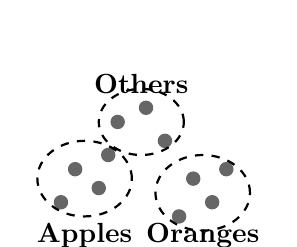
\begin{tikzpicture}[scale=0.6]
        % Red cluster
        \filldraw[black!60] (1.0,1.5) circle (4pt);
        \filldraw[black!60] (1.8,1.8) circle (4pt);
        \filldraw[black!60] (1.3,2.2) circle (4pt);
        \filldraw[black!60] (2.0,2.5) circle (4pt);
        \draw[black, dashed, thick] (1.5,2.0) ellipse (1.0cm and 0.8cm);
        \node[black, font=\bfseries] at (1.5,0.8) {Apples};
        
        % Green cluster
        \filldraw[black!60] (3.5,1.2) circle (4pt);
        \filldraw[black!60] (4.2,1.5) circle (4pt);
        \filldraw[black!60] (3.8,2.0) circle (4pt);
        \filldraw[black!60] (4.5,2.2) circle (4pt);
        \draw[black, dashed, thick] (4.0,1.7) ellipse (1.0cm and 0.8cm);
        \node[black, font=\bfseries] at (4.0,0.8) {Oranges};
        
        % Blue cluster
        \filldraw[black!60] (2.2,3.2) circle (4pt);
        \filldraw[black!60] (2.8,3.5) circle (4pt);
        \filldraw[black!60] (3.2,2.8) circle (4pt);
        \draw[black, dashed, thick] (2.7,3.2) ellipse (0.9cm and 0.7cm);
        \node[black, font=\bfseries] at (2.7,4.0) {Others};
    \end{tikzpicture}
    \caption{Visual representation of clustering: Similar data points are grouped together into distinct clusters. The dashed ellipses represent cluster boundaries.}
    \label{fig:clustering}
\end{figure}

\subsection{Analogy: Sorting a Fruit Basket}

To better understand clustering, consider the simple analogy of sorting a fruit basket. When you have a basket containing various fruits, you naturally group them by type - all apples go in one bowl, all oranges in another, and so on. This intuitive process mirrors exactly what clustering algorithms do computationally: they organize data points into meaningful groups based on their inherent similarities.

\begin{tcolorbox}[title=Analogy]
\centering
\large
Like sorting a fruit basket: all \textbf{apples} go in one bowl, all \textbf{oranges} in another.
\end{tcolorbox}

\subsection{Real-World Problem: Superstore Customer Segmentation}

To illustrate the practical importance of clustering, let us consider a real-world problem faced by many businesses today.

\subsubsection{The Scenario}

A large superstore serves approximately 10,000 customers and wants to better understand their customer base. The store has collected detailed data about each customer, including:

\begin{itemize}
    \item \textbf{Age}: Numerical values such as 25, 30, 45, 50 years, etc.
    \item \textbf{Monthly Expense}: Purchase amounts ranging from \$100 to \$1000 or more.
    \item \textbf{Shopping Preferences}: Categories of products purchased including Electronics, Grocery, Fashion, etc.
\end{itemize}

\subsubsection{The Challenge}

The store's management wants to create targeted marketing offers for different customer segments. For example, they might want to offer student discounts to young customers with limited budgets, family combo packs to middle-aged customers buying groceries, or premium membership benefits to high-spending customers.

However, manually grouping 10,000 customers based on these multiple attributes is practically impossible. Even if attempted, manual grouping would be time-consuming, subjective, and likely to miss subtle patterns in the data.

\begin{tcolorbox}[title=The Central Question]
\centering
\Large
\textbf{How can they group these customers to create targeted offers for each group?}
\end{tcolorbox}

\begin{figure}[H]
    \centering
    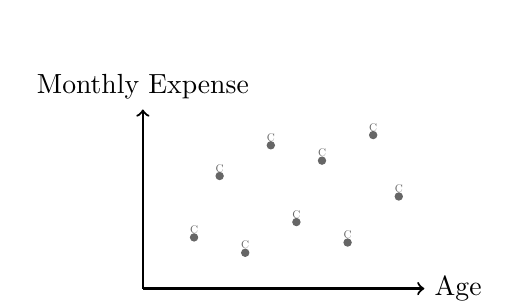
\begin{tikzpicture}[scale=0.65]
        \draw[->, thick] (0,0) -- (5.5,0) node[right] {Age};
        \draw[->, thick] (0,0) -- (0,3.5) node[above] {Monthly Expense};
        
        \foreach \x/\y in {1/1.0, 1.5/2.2, 2/0.7, 2.5/2.8, 3/1.3, 3.5/2.5, 4/0.9, 4.5/3.0, 5/1.8} {
            \filldraw[black!60] (\x,\y) circle (2pt) node[above, scale=0.4] {C};
        }
    \end{tikzpicture}
    \caption{Scatter plot of customer data showing Age vs. Monthly Expense. Each 'C' represents a customer. Without clustering, the data appears as an unstructured collection of points.}
    \label{fig:scattered}
\end{figure}

\subsection{Solution: Clustering}

Clustering provides an elegant solution to this problem. By applying a clustering algorithm to the customer data, the superstore can automatically identify natural groupings of customers based on their age, spending habits, and preferences.

\subsubsection{What is a Cluster?}

When clustering is applied to the customer data, the algorithm forms groups called \textbf{clusters}. Each cluster consists of customers who share similar characteristics. For example, one cluster might contain young customers with low monthly expenses, while another might contain older customers with high spending.

\begin{tcolorbox}[title=Definition]
\centering
Each group formed by clustering is called a \textbf{Cluster}.
\end{tcolorbox}

\subsubsection{The Three Customer Segments}

In our superstore example, the clustering algorithm identifies three distinct customer segments:

\begin{enumerate}
    \item \textbf{Students}: Young customers with low monthly expenses. They are likely students or early-career professionals with limited disposable income.
    
    \item \textbf{Families}: Middle-aged customers with moderate monthly expenses. They are likely families purchasing groceries and household items regularly.
    
    \item \textbf{Premium}: Older customers with high monthly expenses. They are likely affluent individuals who value quality and exclusive products.
\end{enumerate}

\begin{figure}[H]
    \centering
    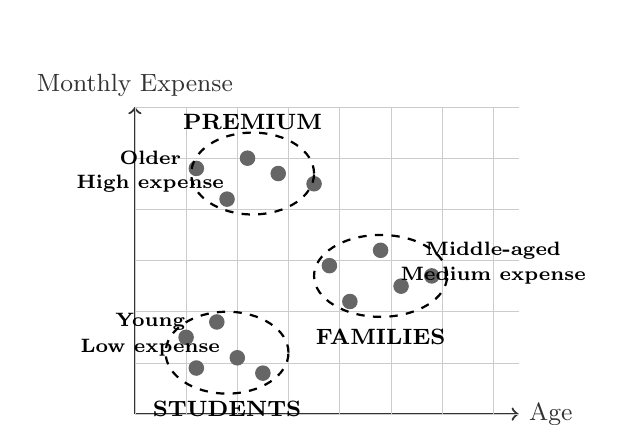
\begin{tikzpicture}[scale=0.65]
        % Draw axes
        \draw[->, thick, black!80] (0,0) -- (7.5,0) node[right, font=\small] {Age};
        \draw[->, thick, black!80] (0,0) -- (0,6.0) node[above, font=\small] {Monthly Expense};
        \draw[very thin, black!20] (0,0) grid (7.5,6.0);
        
        % ============================================================
        % STUDENTS Cluster - Bottom Left
        % ============================================================
        \filldraw[black!60] (1.2,0.9) circle (4pt);
        \filldraw[black!60] (2.0,1.1) circle (4pt);
        \filldraw[black!60] (1.6,1.8) circle (4pt);
        \filldraw[black!60] (2.5,0.8) circle (4pt);
        \filldraw[black!60] (1.0,1.5) circle (4pt);
        
        \draw[black, dashed, thick] (1.8,1.2) ellipse (1.2cm and 0.8cm);
        \node[black, font=\bfseries\footnotesize] at (1.8,0.1) {STUDENTS};
        
        \node[black, font=\scriptsize\bfseries] at (0.3,1.8) {Young};
        \node[black, font=\scriptsize\bfseries] at (0.3,1.3) {Low expense};
        
        % ============================================================
        % FAMILIES Cluster - Middle Right
        % ============================================================
        \filldraw[black!60] (4.2,2.2) circle (4pt);
        \filldraw[black!60] (5.2,2.5) circle (4pt);
        \filldraw[black!60] (4.8,3.2) circle (4pt);
        \filldraw[black!60] (5.8,2.7) circle (4pt);
        \filldraw[black!60] (3.8,2.9) circle (4pt);
        
        \draw[black, dashed, thick] (4.8,2.7) ellipse (1.3cm and 0.8cm);
        \node[black, font=\bfseries\footnotesize] at (4.8,1.5) {FAMILIES};
        
        \node[black, font=\scriptsize\bfseries] at (7.0,3.2) {Middle-aged};
        \node[black, font=\scriptsize\bfseries] at (7.0,2.7) {Medium expense};
        
        % ============================================================
        % PREMIUM Cluster - Top Left
        % ============================================================
        \filldraw[black!60] (1.8,4.2) circle (4pt);
        \filldraw[black!60] (2.8,4.7) circle (4pt);
        \filldraw[black!60] (3.5,4.5) circle (4pt);
        \filldraw[black!60] (2.2,5.0) circle (4pt);
        \filldraw[black!60] (1.2,4.8) circle (4pt);
        
        \draw[black, dashed, thick] (2.3,4.7) ellipse (1.2cm and 0.8cm);
        \node[black, font=\bfseries\footnotesize] at (2.3,5.7) {PREMIUM};
        
        \node[black, font=\scriptsize\bfseries] at (0.3,5.0) {Older};
        \node[black, font=\scriptsize\bfseries] at (0.3,4.5) {High expense};
        
    \end{tikzpicture}
    \caption{Three distinct customer clusters identified through clustering: Students, Families, and Premium customers.}
    \label{fig:clusters}
\end{figure}

\subsubsection{Targeted Marketing Offers}

Once the clusters are identified, the store can create targeted offers tailored to each segment:

\begin{tcolorbox}[title=Result: Targeted Offers]
\begin{itemize}
    \item \textbf{Students} → Discount on electronics and student-friendly products
    \item \textbf{Families} → Combo offers on groceries and family packs
    \item \textbf{Premium} → Exclusive membership benefits and luxury items
\end{itemize}
\end{tcolorbox}

\begin{tcolorbox}[title=Key Insight]
\centering
\large
\textbf{Each cluster contains customers with similar characteristics!}
\end{tcolorbox}

\subsection{Limitations of Regular Clustering}

While the clustering solution successfully identifies customer groups, it has a fundamental limitation: it produces \textbf{flat partitions}. In other words, regular clustering tells us which group each customer belongs to, but it does not reveal any hierarchical relationships between the groups.

\begin{tcolorbox}[title=What's Missing?]
\centering
\Large
Regular clustering gives us \textbf{groups}... \\[0.3cm]
But it doesn't tell us \textbf{how groups are related} to each other! \\[0.3cm]
\textbf{We need something more...}
\end{tcolorbox}

Consider these questions that regular clustering cannot answer:
\begin{itemize}
    \item Are the "Students" and "Families" clusters more similar to each other than either is to "Premium"?
    \item Can we create a hierarchy of clusters (e.g., combining Students and Families into a "Moderate Spenders" super-cluster)?
    \item At what level of similarity do these groups merge?
\end{itemize}

This is where \textbf{Hierarchical Clustering} comes into play.

\section{Definition of Hierarchical Clustering}

Hierarchical clustering is a type of clustering technique used to group similar data points into clusters while maintaining a hierarchical structure. It is also known as Hierarchical Cluster Analysis (HCA). This method constructs a tree-like structure called a dendrogram, which represents the relationships between different clusters based on their similarity.

Unlike traditional clustering methods, hierarchical clustering not only groups the data but also shows how the clusters are related to each other at different levels. This makes it easier to understand the structure of the data and identify meaningful patterns.

\section{Dendrogram}

A dendrogram is a graphical representation of hierarchical clustering. It shows how data points are merged or split at different stages of the clustering process.

In a dendrogram:
\begin{itemize}
    \item Each leaf node represents an individual data point
    \item Branches represent the merging of clusters
    \item The height indicates the distance or dissimilarity between clusters
\end{itemize}

This visualization helps in deciding the number of clusters by cutting the dendrogram at a certain level.

\begin{figure}
    \centering
    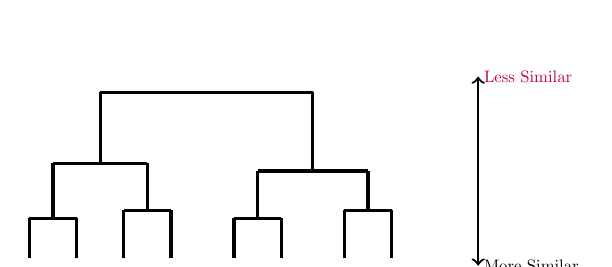
\begin{tikzpicture}
    
        \draw[black,very thick] (0.8,0.6) -- (1.4,0.6);
        \draw[black,very thick] (0.8,0.6) -- (0.8,0.1);
        \draw[black,very thick] (1.4,0.6) -- (1.4,0.1);
    
        \draw[black,very thick] (2.0,0.7) -- (2.6,0.7);
        \draw[black,very thick] (2.0,0.7) -- (2.0,0.1);
        \draw[black,very thick] (2.6,0.7) -- (2.6,0.1);
        \draw[black,very thick] (3.4,0.6) -- (4.0,0.6);
        \draw[black,very thick] (3.4,0.6) -- (3.4,0.1);
        \draw[black,very thick] (4.0,0.6) -- (4.0,0.1);
    
                
        \draw[black,very thick] (4.8,0.7) -- (5.4,0.7);
        \draw[black,very thick] (4.8,0.7) -- (4.8,0.1);
        \draw[black,very thick] (5.4,0.7) -- (5.4,0.1);
    
                
        \draw[black,very thick] (1.1,1.3) -- (2.3,1.3);
        \draw[black,very thick] (1.1,1.3) -- (1.1,0.6);
        \draw[black,very thick] (2.3,1.3) -- (2.3,0.7);
    
                
        \draw[black,very thick] (3.7,1.2) -- (5.1,1.2);
        \draw[black,very thick] (3.7,1.2) -- (3.7,0.6);
        \draw[black,very thick] (5.1,1.2) -- (5.1,0.7);
    
        \draw[black,very thick] (1.7,2.2) -- (4.4,2.2);
        \draw[black,very thick] (1.7,2.2) -- (1.7,1.3);
        \draw[black,very thick] (4.4,2.2) -- (4.4,1.2);
    
        \draw[<->,thick] (6.5,0) -- (6.5,2.4);
        \node[purple,right,scale=0.6] at (6.5,2.4) {Less Similar};
        \node[black,right,scale=0.6] at (6.5,0) {More Similar};
            
    \end{tikzpicture}
    \caption{Dendrogram}
    \label{fig:Dendrogram}
\end{figure}

\section{Types of Hierarchical Clustering}

Hierarchical clustering can be divided into two main types:

\subsection{Agglomerative Clustering (Bottom-Up Approach)}

Agglomerative clustering is the most commonly used hierarchical clustering method. It follows a bottom-up approach where each data point initially starts as an individual cluster. Then, the closest clusters are merged step by step until all data points are grouped into a single cluster.

The process can be described as follows:
\begin{enumerate}
    \item Start with each data point as a separate cluster
    \item Find the two closest clusters
    \item Merge them into a single cluster
    \item Repeat the process until only one cluster remains
\end{enumerate}

This method is simple and widely used because of its computational efficiency.

\subsection{Agglomerative Clustering Example}

In this example, several data points are considered, and the Euclidean distance is used to measure similarity between them.

Initially, each point is treated as a separate cluster. Then, the closest points are merged step by step. Gradually, small clusters are combined into larger clusters until all points belong to a single cluster. This process forms a hierarchical structure that can be visualized using a dendrogram.


\begin{figure}
    \centering
    \begin{subfigure}{0.45\textwidth}
        \centering
        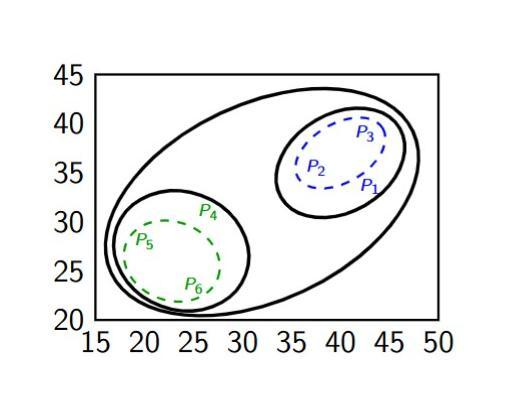
\includegraphics[width=\linewidth]{images/before_clustering.jpg}
        \caption{Data without clustering}
    \end{subfigure}
    \hfill
    \begin{subfigure}{0.45\textwidth}
        \centering
        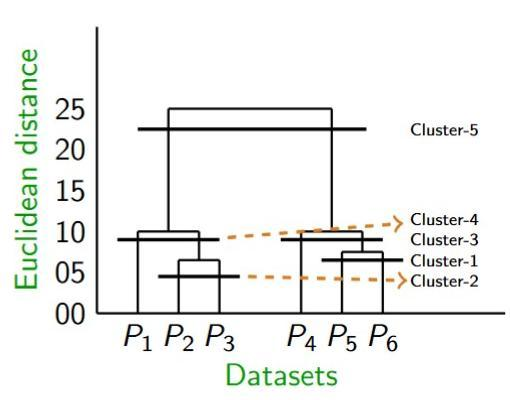
\includegraphics[width=\linewidth]{images/after_clustering.jpg}
        \caption{Data after clustering}
    \end{subfigure}
    
    \caption{Agglomerative Clustering Example}
    \label{fig:agglo_example}
\end{figure}

\subsection{Divisive Clustering (Top-Down Approach)}

Divisive clustering follows the opposite approach of agglomerative clustering. It starts with all data points grouped into a single cluster and then divides them into smaller clusters step by step.

The process can be described as follows:
\begin{enumerate}
    \item Start with all data points in one cluster
    \item Split the cluster into two smaller clusters
    \item Continue splitting until each data point becomes its own cluster
\end{enumerate}

Although divisive clustering is conceptually simple, it is less commonly used due to its higher computational complexity.

\section{Comparison of Approaches}

Among the two approaches, agglomerative clustering is more widely used in practice because it is simpler and computationally more efficient compared to divisive clustering.

% ============================================================
\section{Linkage Criteria}

When performing hierarchical clustering, a key question arises: how do we define the ``closeness'' or distance between two clusters (as opposed to two individual points)? The answer depends on the \textbf{linkage method} chosen. Different linkage criteria lead to different cluster shapes and hierarchical structures.

There are four major linkage methods:

\begin{itemize}
    \item \textbf{Single Linkage (Min):} Distance is defined as the minimum distance between any pair of points from the two clusters. This can lead to a ``chaining'' effect, producing long, thin clusters.
    \item \textbf{Complete Linkage (Max):} Distance is defined as the maximum distance between any pair of points from the two clusters. This tends to produce compact, spherical clusters.
    \item \textbf{Average Linkage (Mean):} Distance is defined as the average of all pairwise distances between points in the two clusters. This is considered a robust middle-ground approach.
    \item \textbf{Ward's Method:} Instead of measuring a distance directly, this method merges the pair of clusters that minimizes the increase in total within-cluster variance ($\Delta$SSE). It is the most popular method for balanced, well-separated data.
\end{itemize}

% ============================================================
\section{Single Linkage Clustering}

\subsection{Definition}

Single linkage (also called the \textit{nearest-neighbor} method) defines the distance between two clusters $C_i$ and $C_j$ as the distance between their closest pair of points:

\[
D(C_i, C_j) = \min_{x \in C_i,\; y \in C_j} d(x, y)
\]

\subsection{Step-by-Step Example}

Consider four data points A, B, C, D with the following pairwise distance matrix:

\[
\begin{array}{c|cccc}
    & A & B & C & D \\
\hline
A & 0 & 2 & 6 & 10 \\
B & 2 & 0 & 5 & 9  \\
C & 6 & 5 & 0 & 4  \\
D & 10 & 9 & 4 & 0  \\
\end{array}
\]

\begin{enumerate}
    \item \textbf{Step 1 -- Find minimum distance:} The smallest entry is $d(A,B) = 2$. Merge A and B into cluster $\{AB\}$.
    \[
    \begin{array}{c|cccc}
        & A & B & C & D \\
    \hline
    A & 0 & \cellcolor{highlight}2 & 6 & 10 \\
    B & \cellcolor{highlight}2 & 0 & 5 & 9  \\
    C & 6 & 5 & 0 & 4  \\
    D & 10 & 9 & 4 & 0  \\
    \end{array}
    \]

    \item \textbf{Step 2 -- Update distance matrix:} Using single linkage, the distance from $\{AB\}$ to each remaining point is the \emph{minimum} of the original distances:
    \[
    \begin{array}{c|ccc}
        & AB & C & D \\
    \hline
    AB & 0 & \min(6,5)=5 & \min(10,9)=9 \\
    C  & 5 & 0 & \cellcolor{highlight}4 \\
    D  & 9 & \cellcolor{highlight}4 & 0 \\
    \end{array}
    \]
    The next minimum is $d(C,D) = 4$. Merge C and D into $\{CD\}$.

    \item \textbf{Step 3 -- Final merge:} Only two clusters remain, $\{AB\}$ and $\{CD\}$:
    \[
    \begin{array}{c|cc}
        & AB & CD \\
    \hline
    AB & 0 & \cellcolor{highlight}{\min(5,9)=5} \\
    CD & \cellcolor{highlight}5 & 0 \\
    \end{array}
    \]
    Merge at height 5.
\end{enumerate}

\subsection{Resulting Dendrogram}

\begin{figure}[h]
    \centering
    \begin{tikzpicture}[x=1.2cm, y=0.6cm, font=\small]
        \foreach \x/\name in {1/A, 2/B, 3/C, 4/D}
            \node at (\x, 0) [below] {\name};
        % A-B merge at height 2
        \draw (1,0) -- (1,2) -- (2,2) -- (2,0);
        \node at (1.5,2) [left] {2};
        % C-D merge at height 4
        \draw (3,0) -- (3,4) -- (4,4) -- (4,0);
        \node at (3.5,4) [right] {4};
        % Final merge at height 5
        \draw (1.5,2) -- (1.5,5) -- (3.5,5) -- (3.5,4);
        \node at (2.5,5) [above] {5};
    \end{tikzpicture}
    \caption{Single Linkage Dendrogram}
    \label{fig:single_linkage_dendrogram}
\end{figure}

% ============================================================
\section{Complete Linkage Clustering}

\subsection{Definition}

Complete linkage (also called the \textit{farthest-neighbor} method) defines the distance between two clusters as the distance between their \emph{farthest} pair of points:

\[
D(C_i, C_j) = \max_{x \in C_i,\; y \in C_j} d(x, y)
\]

\subsection{Step-by-Step Example}

Using the same distance matrix as before:

\begin{enumerate}
    \item \textbf{Step 1 -- Find minimum distance:} Same as single linkage, the smallest entry is $d(A,B) = 2$. Merge A and B.
    \[
    \begin{array}{c|cccc}
        & A & B & C & D \\
    \hline
    A & 0 & \cellcolor{highlight}2 & 6 & 10 \\
    B & \cellcolor{highlight}2 & 0 & 5 & 9  \\
    C & 6 & 5 & 0 & 4  \\
    D & 10 & 9 & 4 & 0  \\
    \end{array}
    \]

    \item \textbf{Step 2 -- Update distance matrix:} Using complete linkage, the distance from $\{AB\}$ to each remaining point is the \emph{maximum}:
    \[
    \begin{array}{c|ccc}
        & AB & C & D \\
    \hline
    AB & 0 & \max(6,5)=6 & \max(10,9)=10 \\
    C  & 6 & 0 & \cellcolor{highlight}4 \\
    D  & 10 & \cellcolor{highlight}4 & 0 \\
    \end{array}
    \]
    The next minimum is $d(C,D) = 4$. Merge C and D.

    \item \textbf{Step 3 -- Final merge:}
    \[
    \begin{array}{c|cc}
        & AB & CD \\
    \hline
    AB & 0 & \cellcolor{highlight}{\max(6,10)=10} \\
    CD & \cellcolor{highlight}{10} & 0 \\
    \end{array}
    \]
    Merge at height 10.
\end{enumerate}

\subsection{Resulting Dendrogram}

\begin{figure}[h]
    \centering
    \begin{tikzpicture}[x=1.2cm, y=0.3cm, font=\small]
        \foreach \x/\name in {1/A, 2/B, 3/C, 4/D}
            \node at (\x, 0) [below] {\name};
        % A-B merge at height 2
        \draw (1,0) -- (1,2) -- (2,2) -- (2,0);
        \node at (1.5,2) [left] {2};
        % C-D merge at height 4
        \draw (3,0) -- (3,4) -- (4,4) -- (4,0);
        \node at (3.5,4) [right] {4};
        % Final merge at height 10
        \draw (1.5,2) -- (1.5,10) -- (3.5,10) -- (3.5,4);
        \node at (2.5,10) [above] {10};
    \end{tikzpicture}
    \caption{Complete Linkage Dendrogram}
    \label{fig:complete_linkage_dendrogram}
\end{figure}

% ============================================================
\section{Average Linkage Clustering}

\subsection{Definition}

Average linkage defines the distance between two clusters as the average of all pairwise distances between points in the two clusters:

\[
D(C_i, C_j) = \frac{1}{|C_i| \cdot |C_j|} \sum_{x \in C_i} \sum_{y \in C_j} d(x, y)
\]

\subsection{Step-by-Step Example}

\begin{enumerate}
    \item \textbf{Step 1:} Minimum distance is $d(A,B) = 2$. Merge A and B.
    \[
    \begin{array}{c|cccc}
        & A & B & C & D \\
    \hline
    A & 0 & \cellcolor{highlight}2 & 6 & 10 \\
    B & \cellcolor{highlight}2 & 0 & 5 & 9  \\
    C & 6 & 5 & 0 & 4  \\
    D & 10 & 9 & 4 & 0  \\
    \end{array}
    \]

    \item \textbf{Step 2 -- Update with averages:}
    \[
    \begin{array}{c|ccc}
        & AB & C & D \\
    \hline
    AB & 0 & \frac{6+5}{2} = 5.5 & \frac{10+9}{2} = 9.5 \\
    C  & 5.5 & 0 & \cellcolor{highlight}4 \\
    D  & 9.5 & \cellcolor{highlight}4 & 0 \\
    \end{array}
    \]
    The next minimum is $d(C,D) = 4$. Merge C and D.

    \item \textbf{Step 3 -- Final merge:}
    \[
    \begin{array}{c|cc}
        & AB & CD \\
    \hline
    AB & 0 & \cellcolor{highlight}{\dfrac{6+10+5+9}{4} = 7.5} \\[6pt]
    CD & \cellcolor{highlight}{7.5} & 0 \\
    \end{array}
    \]
    Merge at height 7.5.
\end{enumerate}

\subsection{Resulting Dendrogram}

\begin{figure}[h]
    \centering
    \begin{tikzpicture}[x=1.2cm, y=0.4cm, font=\small]
        \foreach \x/\name in {1/A, 2/B, 3/C, 4/D}
            \node at (\x, 0) [below] {\name};
        % A-B merge at height 2
        \draw (1,0) -- (1,2) -- (2,2) -- (2,0);
        \node at (1.5,2) [left] {2};
        % C-D merge at height 4
        \draw (3,0) -- (3,4) -- (4,4) -- (4,0);
        \node at (3.5,4) [right] {4};
        % Final merge at height 7.5
        \draw (1.5,2) -- (1.5,7.5) -- (3.5,7.5) -- (3.5,4);
        \node at (2.5,7.5) [above] {7.5};
    \end{tikzpicture}
    \caption{Average Linkage Dendrogram}
    \label{fig:average_linkage_dendrogram}
\end{figure}

% ============================================================
\section{Comparison of Linkage Methods}

\subsection{Numerical Comparison}

All three methods start with the same initial distance matrix and make the same first two merges (A--B at height 2, and C--D at height 4). However, they differ in the final merge height:

\begin{itemize}
    \item \textbf{Single Linkage:} Final merge at height $5$ (uses the closest pair).
    \item \textbf{Complete Linkage:} Final merge at height $10$ (uses the farthest pair).
    \item \textbf{Average Linkage:} Final merge at height $7.5$ (uses the mean of all pairs).
\end{itemize}

\subsection{Side-by-Side Dendrogram Comparison}

\begin{figure}[h]
    \centering
    \begin{subfigure}{0.32\textwidth}
        \centering
        \begin{tikzpicture}[x=0.9cm, y=0.2cm, font=\footnotesize]
            \foreach \x/\name in {1/A, 2/B, 3/C, 4/D}
                \node at (\x, 0) [below] {\name};
            \draw (1,0)--(1,2)--(2,2)--(2,0);
            \node at (1.5,2) [left] {\tiny 2};
            \draw (3,0)--(3,4)--(4,4)--(4,0);
            \node at (3.5,4) [right] {\tiny 4};
            \draw (1.5,2)--(1.5,5)--(3.5,5)--(3.5,4);
            \node at (2.5,5) [above] {\tiny 5};
        \end{tikzpicture}
        \caption{Single Linkage}
    \end{subfigure}
    \hfill
    \begin{subfigure}{0.32\textwidth}
        \centering
        \begin{tikzpicture}[x=0.9cm, y=0.1cm, font=\footnotesize]
            \foreach \x/\name in {1/A, 2/B, 3/C, 4/D}
                \node at (\x, 0) [below] {\name};
            \draw (1,0)--(1,2)--(2,2)--(2,0);
            \node at (1.5,2) [left] {\tiny 2};
            \draw (3,0)--(3,4)--(4,4)--(4,0);
            \node at (3.5,4) [right] {\tiny 4};
            \draw (1.5,2)--(1.5,10)--(3.5,10)--(3.5,4);
            \node at (2.5,10) [above] {\tiny 10};
        \end{tikzpicture}
        \caption{Complete Linkage}
    \end{subfigure}
    \hfill
    \begin{subfigure}{0.32\textwidth}
        \centering
        \begin{tikzpicture}[x=0.9cm, y=0.15cm, font=\footnotesize]
            \foreach \x/\name in {1/A, 2/B, 3/C, 4/D}
                \node at (\x, 0) [below] {\name};
            \draw (1,0)--(1,2)--(2,2)--(2,0);
            \node at (1.5,2) [left] {\tiny 2};
            \draw (3,0)--(3,4)--(4,4)--(4,0);
            \node at (3.5,4) [right] {\tiny 4};
            \draw (1.5,2)--(1.5,7.5)--(3.5,7.5)--(3.5,4);
            \node at (2.5,7.5) [above] {\tiny 7.5};
        \end{tikzpicture}
        \caption{Average Linkage}
    \end{subfigure}
    \caption{Comparison of Single, Complete, and Average Linkage Dendrograms}
    \label{fig:comparison_dendrograms}
\end{figure}

\subsection{Qualitative Comparison}

\begin{center}
\begin{tabular}{|l|l|l|l|}
\hline
\textbf{Method} & \textbf{Distance Used} & \textbf{Cluster Shape} & \textbf{Sensitivity} \\
\hline
Single Linkage  & Minimum pair & Long, chained & Sensitive to outliers \\
Complete Linkage & Maximum pair & Compact, spherical & Less sensitive \\
Average Linkage  & Mean of all pairs & Balanced & Robust middle ground \\
Ward's Method    & Min $\Delta$SSE & Balanced, equal-sized & Best for compact clusters \\
\hline
\end{tabular}
\end{center}

% ============================================================
\section{The Dendrogram: A Visual Hierarchy}

A dendrogram is more than just a diagram -- it encodes the entire history of the clustering process in a single tree structure. Its key components are:

\begin{itemize}
    \item \textbf{Leaves:} Individual data points, shown at the bottom (or left) of the tree.
    \item \textbf{Branches:} Internal nodes that represent groups formed as similar data points are merged together at successive steps.
    \item \textbf{Root:} The topmost node where all data points are united into a single cluster.
    \item \textbf{Height:} The vertical position at which two branches join. A higher join indicates that the two clusters were more dissimilar when merged.
\end{itemize}

\begin{figure}[h]
    \centering
    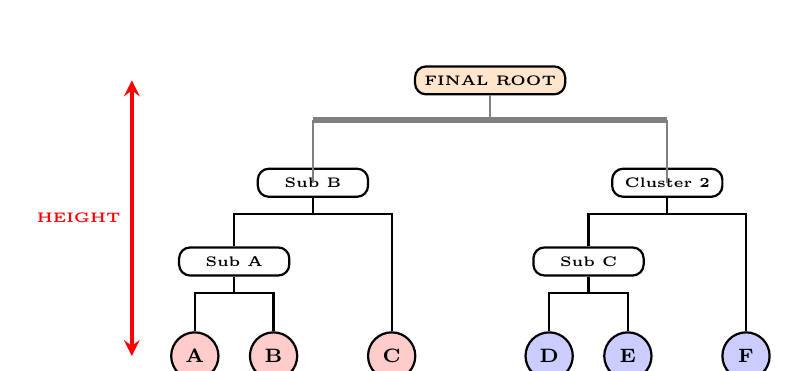
\begin{tikzpicture}[
        leaf/.style={circle, draw, thick, minimum size=0.6cm, font=\scriptsize\bfseries,
                     inner sep=1pt, fill=red!20},
        branch/.style={rectangle, rounded corners, draw, thick, minimum width=1.4cm,
                       font=\tiny\bfseries, fill=white},
        line/.style={thick}
    ]
        % Leaves
        \node[leaf] (A) at (0,0) {A};
        \node[leaf] (B) at (1,0) {B};
        \node[leaf] (C) at (2.5,0) {C};
        \node[leaf, fill=blue!20] (D) at (4.5,0) {D};
        \node[leaf, fill=blue!20] (E) at (5.5,0) {E};
        \node[leaf, fill=blue!20] (F) at (7,0) {F};

        % Sub-branches
        \draw[line] (A) -- (0,0.8) -- (1,0.8) -- (B);
        \node[branch] (SubA) at (0.5,1.2) {Sub A};
        \draw[line] (0.5,0.8) -- (SubA);

        \draw[line] (D) -- (4.5,0.8) -- (5.5,0.8) -- (E);
        \node[branch] (SubC) at (5,1.2) {Sub C};
        \draw[line] (5,0.8) -- (SubC);

        % Higher branches
        \draw[line] (SubA) -- (0.5,1.8) -- (2.5,1.8) -- (C);
        \node[branch] (SubB) at (1.5,2.2) {Sub B};
        \draw[line] (1.5,1.8) -- (SubB);

        \draw[line] (SubC) -- (5,1.8) -- (7,1.8) -- (F);
        \node[branch] (Clust2) at (6,2.2) {Cluster 2};
        \draw[line] (6,1.8) -- (Clust2);

        % Root
        \draw[line, gray, line width=2pt] (1.5,3) -- (6,3);
        \draw[line, gray] (1.5,2.2) -- (1.5,3);
        \draw[line, gray] (6,2.2) -- (6,3);
        \node[branch, fill=orange!20] (Root) at (3.75,3.5) {FINAL ROOT};
        \draw[line, gray] (3.75,3) -- (Root);

        % Height arrow
        \draw[<->, >=stealth, red, line width=1.5pt]
            (-0.8,0) -- (-0.8,3.5)
            node[midway, left, font=\tiny\bfseries] {HEIGHT};
    \end{tikzpicture}
    \caption{Structure of a Dendrogram}
    \label{fig:dendrogram_structure}
\end{figure}

By cutting the dendrogram at a chosen height, the analyst can select the number of clusters that best suits the problem at hand. A cut at a low height produces many small clusters, while a cut at a high height produces fewer, larger clusters.

\end{document}